%
% 02_Grundlagen.tex -- Ellipsengeometrie, Drehimpulserhaltung,
% Bahngleichung und die Umlaufzeit als Integral
%
% !TEX root = ../../buch.tex
% !TEX encoding = UTF-8
%
\section{Geometrische und physikalische Grundlagen
\label{kepler:section:grundlagen}}
\kopfrechts{Geometrische und physikalische Grundlagen}%

Für die Umlaufzeit eines Planeten brauchen wir zwei Zutaten.
Die erste Zutat ist die geometrische Form der Bahn.
Die zweite Zutat ist die Geschwindigkeit, mit der der Planet diese Bahn durchläuft.
Die Form liefert das erste keplersche Gesetz.
Die Geschwindigkeit liefert das zweite.
In diesem Abschnitt beschreiben wir zuerst die Ellipse in Polarkoordinaten.
Dann leiten wir beide Gesetze aus der newtonschen Mechanik her.
Daraus gewinnen wir eine Integraldarstellung der Umlaufzeit.
Diese Darstellung ist der Ausgangspunkt für alles Weitere.

\subsection{Die Ellipse in Polarkoordinaten
\label{kepler:subsection:ellipse}}

\begin{figure}
\centering
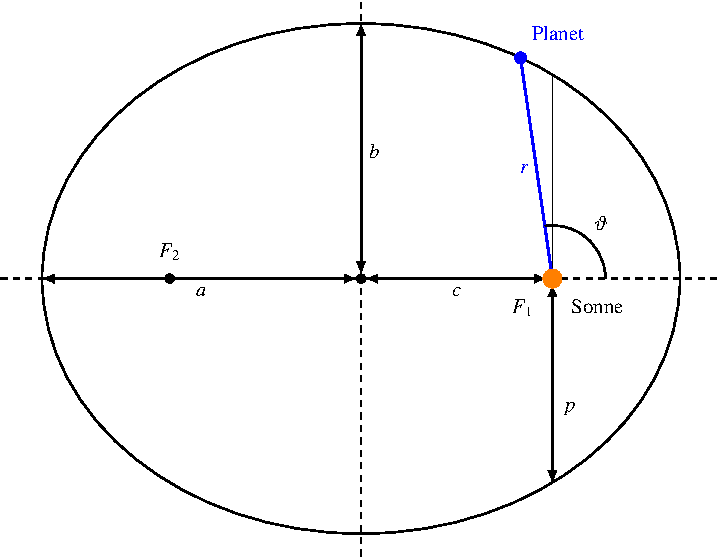
\includegraphics{papers/kepler/images/bahn.pdf}
\caption{Bahnellipse eines Planeten mit grosser Halbachse $a$ und
kleiner Halbachse $b$.
Die Sonne steht im Brennpunkt $F_1$.
Der zweite Brennpunkt $F_2$ bleibt leer.
Die Brennpunkte liegen im Abstand $c$ vom Mittelpunkt der Ellipse.
Der Halbparameter $p$ wird senkrecht zur grossen Achse gemessen.
Die durchgezogene Sehne durch $F_1$ liegt symmetrisch zur grossen Achse und steht deshalb senkrecht auf ihr.
Der Ort des Planeten wird durch den Abstand $r$ zur Sonne und den Polarwinkel $\vartheta$ beschrieben.
Der Winkel wird vom sonnennächsten Punkt aus gemessen.
\label{kepler:figure:ellipse}}
\end{figure}


Eine Ellipse hat eine grosse Halbachse $a$ und eine kleine Halbachse $b$.
\index{Halbachse}%
Sie besitzt zwei Brennpunkte $F_1$ und $F_2$.
\index{Brennpunkt}%
Diese liegen auf der grossen Achse im Abstand $c=\!\sqrt{a^2-b^2}$ vom Mittelpunkt (Abbildung~\ref{kepler:figure:ellipse}).
Das Verhältnis
\begin{equation}
\varepsilon
=
\frac{c}{a}
=
\!\sqrt{1-\frac{b^2}{a^2}}
\label{kepler:eqn:exzentrizitaet}
\end{equation}
heisst \emph{numerische Exzentrizität}.
\index{Exzentriztität, numerisch}%
Sie misst die Abweichung von der Kreisform.
Für eine Ellipse gilt $0\le \varepsilon<1$.
Der Grenzfall $\varepsilon=0$ ergibt einen Kreis.
Wir schreiben die Exzentrizität mit dem griechischen Buchstaben $\varepsilon$.
\index{epsilon@$\varepsilon$}%
Das reguläre $e$ bleibt so für die eulersche Zahl reserviert.
\index{e@$e$}%
\index{eulersche Zahl}%

Für die Rechnung eignen sich Polarkoordinaten $(r,\vartheta)$ am besten.
\index{Polarkoordinaten}%
Die Sonne liegt dabei im Ursprung, also im Brennpunkt $F_1$.
\index{Sonne}%
In diesen Koordinaten lautet die Gleichung der Ellipse
\begin{equation}
r(\vartheta)
=
\frac{p}{1+\varepsilon\cos(\vartheta)}
\qquad\text{mit}\qquad
p
=
\frac{b^2}{a}
=
a(1-\varepsilon^2).
\label{kepler:eqn:ellipse}
\end{equation}
Die Grösse $p$ heisst \emph{Halbparameter} der Ellipse.
\index{Halbparameter}%
\index{p@$p$}%
Sie ist der Abstand von der Sonne zur Bahn senkrecht zur grossen Achse.
Der Winkel $\vartheta$ wird vom sonnennächsten Punkt aus gemessen.
Für $\vartheta=0$ ist der Nenner maximal und der Abstand $r$ minimal.
Für $\vartheta=\pi$ erreicht der Planet den sonnenfernsten Punkt.
In Abschnitt~\ref{kepler:subsection:bahngleichung} leiten wir diese
Bahnform aus der Bewegungsgleichung her.

\subsection{Drehimpulserhaltung und der Flächensatz
\label{kepler:subsection:flaechensatz}}

Die Sonne habe die Masse $M$ und der Planet die Masse $m$.
Nach Newton \cite{kepler:principia} ist die Gravitationskraft
\begin{equation}
\vec{F}
=
-\frac{GMm}{r^2}\,\hat{r}.
\label{kepler:eqn:gravitation}
\end{equation}
Dabei ist $G$ die Gravitationskonstante.
Der Vektor $\hat{r}$ ist der Einheitsvektor von der Sonne zum Planeten.
Die Gravitation ist eine Zentralkraft.
\index{Zentralkraft}%
Sie wirkt immer entlang der Verbindungslinie von Sonne und Planet.
Deshalb verschwindet das Drehmoment bezüglich der Sonne: Wegen
$\vec{F}\parallel\vec{r}$ gilt $\vec{r}\times\vec{F}=0$.
Das Drehmoment ist die zeitliche Änderung des Drehimpulses.
\index{Drehmoment}%
Der Drehimpuls
\index{Drehimpuls}%
\begin{equation}
\vec{L}
=
m\,(\vec{r}\times\vec{v})
=
\text{konstant}
\label{kepler:eqn:drehimpulsvektor}
\end{equation}
bleibt deshalb während der ganzen Bewegung erhalten.
Daraus folgt auch, dass die Bahn eben ist.
Der Ortsvektor $\vec{r}$ steht nämlich immer senkrecht auf dem festen Vektor $\vec{L}$.
Wir können die Bewegung deshalb vollständig in der Bahnebene beschreiben.
\index{Bahnebene}%
Dazu verwenden wir die Polarkoordinaten aus Abschnitt~\ref{kepler:subsection:ellipse}.

In Polarkoordinaten hat die Geschwindigkeit zwei Komponenten.
Die radiale Komponente ist $\dot{r}$.
Die dazu senkrechte Komponente ist $r\dot{\vartheta}$.
Zum Kreuzprodukt in \eqref{kepler:eqn:drehimpulsvektor} trägt nur die senkrechte Komponente bei.
Der Betrag des Drehimpulses ist daher
\begin{equation}
L
=
m\,r^2\,\dot{\vartheta}.
\label{kepler:eqn:drehimpuls}
\end{equation}
Diese Beziehung enthält bereits das zweite keplersche Gesetz.
\index{keplersches Gesetz!zweites}%
In einem kurzen Zeitintervall $dt$ überstreicht der Fahrstrahl näherungsweise ein schmales Dreieck.
\index{Fahrstrahl}%
Das Dreieck hat die Seiten $r$ und $r\,d\vartheta$, also die Fläche $dA=\frac12 r^2\,d\vartheta$.
Mit \eqref{kepler:eqn:drehimpuls} folgt für die
Flächengeschwindigkeit
\begin{equation}
\frac{dA}{dt}
=
\frac12\,r^2\,\dot{\vartheta}
=
\frac{L}{2m}
=
\text{konstant}.
\label{kepler:eqn:flaechensatz}
\end{equation}
Der Fahrstrahl überstreicht in gleichen Zeiten also gleich grosse Flächen.
Anschaulich heisst das: In Sonnennähe ist ein Planet schneller als in Sonnenferne.
Für uns ist vor allem die Form \eqref{kepler:eqn:drehimpuls} wichtig.
Sie verknüpft die Winkelgeschwindigkeit $\dot{\vartheta}$ mit dem Abstand $r$.
Damit können wir später die Umlaufzeit als Integral über den Winkel schreiben.

\subsection{Die Bahngleichung
\label{kepler:subsection:bahngleichung}}

Jetzt begründen wir das erste keplersche Gesetz.
Dabei finden wir auch den Zusammenhang zwischen dem Drehimpuls $L$ und der Bahngeometrie.
Diesen Zusammenhang brauchen wir später.

Die Bewegungsgleichung lautet $m\ddot{\vec{r}}=\vec{F}$.
Ihre radiale Komponente ist in Polarkoordinaten
\begin{equation}
\ddot{r}-r\dot{\vartheta}^2
=
-\frac{GM}{r^2}.
\label{kepler:eqn:radialgleichung}
\end{equation}
Der Term $r\dot{\vartheta}^2$ beschreibt die Zentrifugalbeschleunigung.
Diese Differentialgleichung enthält noch die Zeit.
Für die Form der Bahn interessiert uns die Zeit aber gar nicht.
Ein bewährter Trick hilft weiter \cite{kepler:goldstein}.
Wir gehen zur neuen Variablen $u=1/r$ über.
Die Zeitableitungen ersetzen wir mit \eqref{kepler:eqn:drehimpuls} durch Ableitungen nach dem Winkel $\vartheta$.
Aus $\dot{\vartheta}=Lu^2/m$ folgt für die radiale Geschwindigkeit
\begin{align*}
\dot{r}
&=
\frac{dr}{d\vartheta}\,\dot{\vartheta}
=
-\frac{1}{u^2}\,\frac{du}{d\vartheta}\cdot\frac{Lu^2}{m}
=
-\frac{L}{m}\,\frac{du}{d\vartheta}
\\
\intertext{und durch nochmaliges Ableiten für die Beschleunigung}
\ddot{r}
&=
-\frac{L}{m}\,\frac{d^2u}{d\vartheta^2}\,\dot{\vartheta}
=
-\frac{L^2u^2}{m^2}\,\frac{d^2u}{d\vartheta^2}.
\end{align*}
Wir setzen beides zusammen mit $r=1/u$ und $\dot{\vartheta}=Lu^2/m$ in
\eqref{kepler:eqn:radialgleichung} ein:
\[
-\frac{L^2u^2}{m^2}\,\frac{d^2u}{d\vartheta^2}
-
\frac{L^2u^3}{m^2}
=
-GMu^2.
\]
Beide Terme auf der linken Seite haben nun denselben Koeffizienten
$-L^2u^2/m^2$.
Wir dividieren die ganze Gleichung durch diesen Koeffizienten.
Übrig bleibt die lineare Differentialgleichung
\begin{equation}
\frac{d^2u}{d\vartheta^2}+u
=
\frac{GMm^2}{L^2}.
\label{kepler:eqn:binet}
\end{equation}
Sie ist in der Mechanik als \emph{Binet-Gleichung} bekannt
\index{Binet-Gleichung}%
\cite{kepler:goldstein}.

Die allgemeine Lösung der Binet-Gleichung \eqref{kepler:eqn:binet} besteht aus zwei Teilen.
Der erste Teil ist die konstante partikuläre Lösung $GMm^2/L^2$.
Der zweite Teil ist die harmonische Lösung der homogenen Gleichung.
Zusammen ergibt das
\[
u(\vartheta)
=
\frac{GMm^2}{L^2}\bigl(1+\varepsilon\cos(\vartheta-\vartheta_0)\bigr)
\]
mit den Integrationskonstanten $\varepsilon\ge 0$ und $\vartheta_0$.
Wir legen die Richtung $\vartheta_0=0$ auf den sonnennächsten Punkt.
Dann kehren wir zu $r=1/u$ zurück.
So entsteht genau die Ellipsengleichung \eqref{kepler:eqn:ellipse}
mit dem Halbparameter
\begin{equation}
p
=
\frac{L^2}{GMm^2}
\qquad\Leftrightarrow\qquad
L
=
m\sqrt{GMp\mathstrut}.
\label{kepler:eqn:drehimpulsgeometrie}
\end{equation}
Für $0\le \varepsilon<1$ ist die Bahn eine Ellipse.
Das beweist das erste keplersche Gesetz.
\index{keplersches Gesetz!erstes}%
Für $\varepsilon\ge 1$ entstehen Parabeln und Hyperbeln.
\index{Parabel}%
\index{Hyperbel}%
Das sind offene Bahnen von Körpern, die nicht an die Sonne gebunden sind.
Ein Beispiel ist Oumuamua, das erste interstellare Objekt, das 2017 im Sonnensystem entdeckt worden ist.
\index{Oumuamua}%
Seine Bahn hat die Exzentrizität $\varepsilon\approx 1.2$ \cite{kepler:oumuamua}.
Für Planeten spielen solche Bahnen keine Rolle.
Die Beziehung \eqref{kepler:eqn:drehimpulsgeometrie} ist bemerkenswert.
Sie drückt den Drehimpuls allein durch die Massen und die Geometrie der Bahn aus.

\subsection{Die Umlaufzeit als Integral
\label{kepler:subsection:umlaufzeit}}

Jetzt haben wir alles für die Umlaufzeit $T$ beisammen.
Aus \eqref{kepler:eqn:drehimpuls} folgt für das Zeitelement
\[
dt
=
\frac{m}{L}\,r^2\,d\vartheta.
\]
Während eines vollen Umlaufs wächst der Polarwinkel von $0$ bis
$2\pi$.
Die Umlaufzeit ist also
\[
T
=
\frac{m}{L}\int_0^{2\pi} r(\vartheta)^2\,d\vartheta.
\]
Nun setzen wir die Ellipsengleichung \eqref{kepler:eqn:ellipse} ein.
So entsteht die Integraldarstellung
\begin{equation}
T
=
\frac{m\,p^2}{L}
\int_0^{2\pi}
\frac{1}{(1+\varepsilon\cos(\vartheta))^2}
\,d\vartheta.
\label{kepler:eqn:tintegral}
\end{equation}
Damit ist das Problem auf ein bestimmtes Integral zurückgeführt.
Das Integral sieht harmlos aus.
Mit reellen Methoden ist es aber unangenehm.
Wir werten das Integral in Abschnitt~\ref{kepler:section:komplex} deshalb mit komplexer Integration aus.
Zuerst betrachten wir aber den Spezialfall der Kreisbahn.
Dort erhält man das dritte keplersche Gesetz auch ohne dieses Integral.
